%%%%%%%%%%%%%%%%%%%%%%%%%%%%%%%%%%%%%%%%%%%%%%%%%%%%%%%%%%%%%%%%%%%%%%%%%%%%%%%%%%%%%%%%%%%%%%%%%%%%%%%%%%%%%%%%%%%%%%%%%%%%%%%%%%%%%%%%%%%%%%%%%%%%%%%%%%%%%%%%%%%
% Written By Michael Brodskiy
% Class: Fundamentals of Electronics
% Professor: I. Salama
%%%%%%%%%%%%%%%%%%%%%%%%%%%%%%%%%%%%%%%%%%%%%%%%%%%%%%%%%%%%%%%%%%%%%%%%%%%%%%%%%%%%%%%%%%%%%%%%%%%%%%%%%%%%%%%%%%%%%%%%%%%%%%%%%%%%%%%%%%%%%%%%%%%%%%%%%%%%%%%%%%%

\include{Includes.tex}

\title{Pre-Lab 2}
\date{\today}
\author{Michael Brodskiy\\ \small Professor: M. Onabajo}

\begin{document}

\maketitle

\begin{enumerate}

  \item

    Using the equation:

    $$i=I_s\left( e^{v/(nV_T)}-1 \right)$$

    and the given measurements, we may write:

    $$10^{-3}=I_s\left( e^{.62/(n.025)}-1 \right)$$
    $$10^{-2}=I_s\left( e^{.69/(n.025)}-1 \right)$$

    Since the exponential is greater than 1, we may simplify to:

    $$\frac{10^{-3}}{e^{24.8/n}}=I_s$$
    $$\frac{10^{-2}}{e^{27.6/n}}=I_s$$

    $$I_s=.001e^{-\frac{24.8}{n}}$$
    $$I_s=.01e^{-\frac{27.6}{n}}$$

    We can combine the two equations to solve for $n$ and $I_s$:

    $$.001e^{-\frac{24.8}{n}}=.01e^{-\frac{27.6}{n}}$$
    $$e^{-\frac{24.8}{n}}=10e^{-\frac{27.6}{n}}$$
    $$e^{\frac{27.6-24.8}{n}}=10$$
    $$\frac{27.6-24.8}{n}=\ln(10)$$
    $$n=\frac{2.8}{\ln(10)}$$
    $$\boxed{n=1.216}$$

    We then plug this into the earlier equations to find $I_s$:

    $$I_s=.001e^{-24.8/1.216}$$
    $$\boxed{I_s=1.3889\cdot10^{-12}[\si{\ampere}]}$$

    We can verify by using the second equation for $I_s$:

    $$I_s=.01e^{-27.6/1.216}$$
    $$\boxed{I_s=1.3889\cdot10^{-12}[\si{\ampere}]}$$

    It is difficult to measure the current in a reverse bias mode, however, because the diode may reach breakdown voltage by increasing the reverse voltage.

  \item Read through, no questions \textcolor{green}{\checkmark}

  \item Taking the forward voltage of the LEDs as $2[\si{\volt}]$, we can make some relevant calculations, assuming each LED will form a ``branch'' consisting of a resistor, optional Zener diode, and the LED itself. First, using the maximum power, we can calculate the maximum current, starting with the first (red) LED to turn on, per the power specifications:

    $$I_{max}=\frac{6\cdot10^{-2}}{.2}=.3[\si{\ampere}]$$

    Now, we find the resistance value, assuming the maximum input ($24[\si{\volt}]$):

    $$R_{red}=\frac{24-2}{.3}=73.33[\si{\ohm}]$$

    We then cascade this with the next LED to turn on (yellow), and add in a Zener diode so that the LED turns on only after $8[\si{\volt}]$. Using a Zener diode, we can calculate current using the maximum voltage input and power rating:

    $$I_{max}^2=\frac{1}{6}=.1667[\si{\ampere}]$$

    We then find the resistor value:

    $$R_{yel}=\frac{24-8}{.1667}=96[\si{\ohm}]$$

    Repeating the same process for green, but with a $15[\si{\volt}]$ Zener:

    $$I_{max}^3=\frac{1}{15}=.0667[\si{\ampere}]$$
    $$R_{grn}=\frac{24-17}{.0667}=105[\si{\ohm}]$$

    Combining this together, we get:

    \begin{figure}[H]
      \centering
      \tikzset{every picture/.style={line width=0.75pt}} %set default line width to 0.75pt        

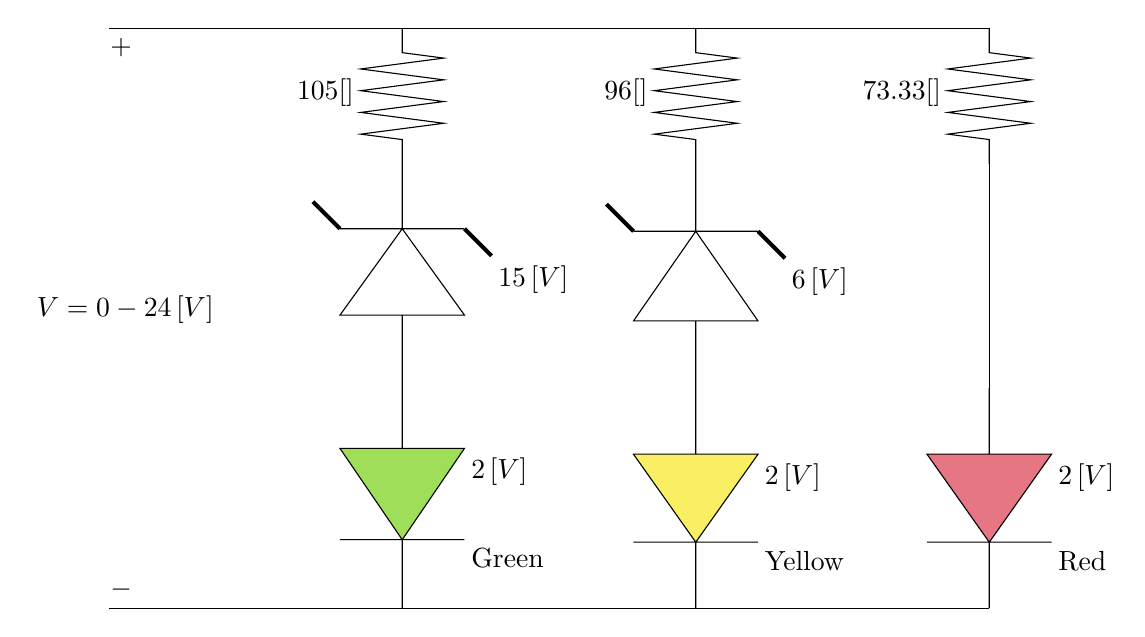
\begin{tikzpicture}[x=0.75pt,y=0.75pt,yscale=-1,xscale=1]
%uncomment if require: \path (0,412); %set diagram left start at 0, and has height of 412

%Shape: Diode [id:dp9916766022166023] 
\draw  [fill={rgb, 255:red, 208; green, 2; blue, 27 }  ,fill opacity=0.54 ] (611,315.8) -- (581,358.2) -- (551,315.8) -- (611,315.8) -- cycle (581,284) -- (581,315.8) (611,358.2) -- (551,358.2) (581,358.2) -- (581,390) ;
%Shape: Diode [id:dp47724199606317685] 
\draw  [fill={rgb, 255:red, 248; green, 231; blue, 28 }  ,fill opacity=0.69 ] (469.58,315.8) -- (439.58,358.2) -- (409.58,315.8) -- (469.58,315.8) -- cycle (439.58,284) -- (439.58,315.8) (469.58,358.2) -- (409.58,358.2) (439.58,358.2) -- (439.58,390) ;
%Straight Lines [id:da43394379079125567] 
\draw    (581,390) -- (439.58,390) ;
%Shape: Resistor [id:dp09973725738727013] 
\draw   (439.58,110.58) -- (439.58,122.35) -- (459.58,124.97) -- (419.58,130.21) -- (459.58,135.44) -- (419.58,140.67) -- (459.58,145.91) -- (419.58,151.14) -- (459.58,156.37) -- (419.58,161.61) -- (439.58,164.22) -- (439.58,176) ;
%Straight Lines [id:da9934104451259984] 
\draw    (581,110.58) -- (439.58,110.58) ;
%Shape: Diode [id:dp30609907031657446] 
\draw  [fill={rgb, 255:red, 126; green, 211; blue, 33 }  ,fill opacity=0.75 ] (328.16,313) -- (298.16,357) -- (268.16,313) -- (328.16,313) -- cycle (298.16,280) -- (298.16,313) (328.16,357) -- (268.16,357) (298.16,357) -- (298.16,390) ;
%Shape: Resistor [id:dp3336013122238709] 
\draw   (298.16,110.58) -- (298.16,122.35) -- (318.16,124.97) -- (278.16,130.21) -- (318.16,135.44) -- (278.16,140.67) -- (318.16,145.91) -- (278.16,151.14) -- (318.16,156.37) -- (278.16,161.61) -- (298.16,164.22) -- (298.16,176) ;
%Straight Lines [id:da4142874846716025] 
\draw    (439.58,390) -- (298.16,390) ;
%Straight Lines [id:da6359356780714503] 
\draw    (298.16,390) -- (156.74,390) ;
%Straight Lines [id:da792670839882941] 
\draw    (439.58,110.58) -- (298.16,110.58) ;
%Straight Lines [id:da5542473757631496] 
\draw    (298.16,110.58) -- (156.74,110.58) ;
%Shape: Diode [id:dp6229217229836789] 
\draw   (268.16,248.8) -- (298.16,207.2) -- (328.16,248.8) -- (268.16,248.8) -- cycle (298.16,280) -- (298.16,248.8) (268.16,207.2) -- (328.16,207.2) (298.16,207.2) -- (298.16,176) ;
%Shape: Diode [id:dp2807840415796292] 
\draw   (409.58,251.6) -- (439.58,208.4) -- (469.58,251.6) -- (409.58,251.6) -- cycle (439.58,284) -- (439.58,251.6) (409.58,208.4) -- (469.58,208.4) (439.58,208.4) -- (439.58,176) ;
%Straight Lines [id:da9880872033365566] 
\draw [line width=1.5]    (255.13,194.17) -- (268.16,207.2) ;
%Straight Lines [id:da4671561501686561] 
\draw [line width=1.5]    (328.16,207.2) -- (341.18,220.23) ;
%Straight Lines [id:da7936008436502483] 
\draw [line width=1.5]    (396.55,195.37) -- (409.58,208.4) ;
%Straight Lines [id:da3769618486887958] 
\draw [line width=1.5]    (469.58,208.4) -- (482.6,221.43) ;
%Straight Lines [id:da15712761589306246] 
\draw    (581,284) -- (581,176) ;
%Shape: Resistor [id:dp44020554709517357] 
\draw   (581,110.58) -- (581,122.35) -- (601,124.97) -- (561,130.21) -- (601,135.44) -- (561,140.67) -- (601,145.91) -- (561,151.14) -- (601,156.37) -- (561,161.61) -- (581,164.22) -- (581,176) ;

% Text Node
\draw (613,361.2) node [anchor=north west][inner sep=0.75pt]   [align=left] {Red};
% Text Node
\draw (471.58,361.2) node [anchor=north west][inner sep=0.75pt]   [align=left] {Yellow};
% Text Node
\draw (330.16,360) node [anchor=north west][inner sep=0.75pt]   [align=left] {Green};
% Text Node
\draw (162.74,113.98) node [anchor=north] [inner sep=0.75pt]    {$+$};
% Text Node
\draw (162.74,386.6) node [anchor=south] [inner sep=0.75pt]    {$-$};
% Text Node
\draw (164.74,246.29) node    {$V=0-24\left[\text{V}\right]$};
% Text Node
\draw (484.6,224.83) node [anchor=north west][inner sep=0.75pt]    {$6\left[\text{V}\right]$};
% Text Node
\draw (471.58,319.2) node [anchor=north west][inner sep=0.75pt]    {$2\left[\text{V}\right]$};
% Text Node
\draw (613,319.2) node [anchor=north west][inner sep=0.75pt]    {$2\left[\text{V}\right]$};
% Text Node
\draw (330.16,316.4) node [anchor=north west][inner sep=0.75pt]    {$2\left[\text{V}\right]$};
% Text Node
\draw (343.18,223.63) node [anchor=north west][inner sep=0.75pt]    {$15\left[\text{V}\right]$};
% Text Node
\draw (559,133.61) node [anchor=north east] [inner sep=0.75pt]    {$73.33[ \si{\ohm}]$};
% Text Node
\draw (417.58,133.61) node [anchor=north east] [inner sep=0.75pt]    {$96[ \si{\ohm}]$};
% Text Node
\draw (276.16,133.61) node [anchor=north east] [inner sep=0.75pt]    {$105[ \si{\ohm}]$};


\end{tikzpicture}

      \caption{Final Configuration}
      \label{fig:1}
    \end{figure}

    Hypothetically, the circuit should be able to operate up to an input voltage of $24[\si{\volt}]$ before the LEDs or Zeners are at threat of burning out or being overloaded.

\end{enumerate}

\end{document}

